%% uncomment to list all files in log
%\listfiles

\documentclass[12pt]{report}


\usepackage{fontspec}

%\setmainfont[Scale=MatchLowercase]{Lucida Bright}
%\setmonofont{FreeMono}
%\setmonofont{Source Code Pro}
\setmonofont[Scale=MatchLowercase]{Ubuntu Mono}

\usepackage[headings]{fullpage}

% national use characters 
%\usepackage{inputenc}

% ams mathematical symbols
\usepackage{amsmath,amssymb}

% added to support pandoc highlighting
\usepackage{microtype}

\usepackage{makeidx}

% add index and bibliographies to table of contents
\usepackage[nottoc]{tocbibind}

% postscript courier and times in place of cm fonts
%\usepackage{courier}
%\usepackage{times}

% extended coloring
\usepackage{color}
\usepackage[table,dvipsnames]{xcolor}
\usepackage{colortbl}

% advanced date formating
\usepackage{datetime}

%support pandoc code highlighting
\usepackage{fancyvrb}
\DefineShortVerb[commandchars=\\\{\}]{\|}
\DefineVerbatimEnvironment{Highlighting}{Verbatim}{commandchars=\\\{\}}
% Add ',fontsize=\small' for more characters per line

%tango style colors
% \usepackage{framed}
% \definecolor{shadecolor}{RGB}{255,255,255}
% \newenvironment{Shaded}{\begin{snugshade}}{\end{snugshade}}
% \newcommand{\KeywordTok}[1]{\textcolor[rgb]{0.13,0.29,0.53}{\textbf{{#1}}}}
% \newcommand{\DataTypeTok}[1]{\textcolor[rgb]{0.13,0.29,0.53}{{#1}}}
% \newcommand{\DecValTok}[1]{\textcolor[rgb]{0.00,0.00,0.81}{{#1}}}
% \newcommand{\BaseNTok}[1]{\textcolor[rgb]{0.00,0.00,0.81}{{#1}}}
% \newcommand{\FloatTok}[1]{\textcolor[rgb]{0.00,0.00,0.81}{{#1}}}
% \newcommand{\CharTok}[1]{\textcolor[rgb]{0.31,0.60,0.02}{{#1}}}
% \newcommand{\StringTok}[1]{\textcolor[rgb]{0.31,0.60,0.02}{{#1}}}
% \newcommand{\CommentTok}[1]{\textcolor[rgb]{0.56,0.35,0.01}{\textit{{#1}}}}
% \newcommand{\OtherTok}[1]{\textcolor[rgb]{0.56,0.35,0.01}{{#1}}}
% \newcommand{\AlertTok}[1]{\textcolor[rgb]{0.94,0.16,0.16}{{#1}}}
% \newcommand{\FunctionTok}[1]{\textcolor[rgb]{0.00,0.00,0.00}{{#1}}}
% \newcommand{\RegionMarkerTok}[1]{{#1}}
% \newcommand{\ErrorTok}[1]{\textbf{{#1}}}
% \newcommand{\NormalTok}[1]{{#1}}

%espresso style colors
% \usepackage{framed}
% \definecolor{shadecolor}{RGB}{42,33,28}
% \newenvironment{Shaded}{\begin{snugshade}}{\end{snugshade}}
% \newcommand{\KeywordTok}[1]{\textcolor[rgb]{0.26,0.66,0.93}{\textbf{{#1}}}}
% \newcommand{\DataTypeTok}[1]{\textcolor[rgb]{0.74,0.68,0.62}{\underline{{#1}}}}
% \newcommand{\DecValTok}[1]{\textcolor[rgb]{0.27,0.67,0.26}{{#1}}}
% \newcommand{\BaseNTok}[1]{\textcolor[rgb]{0.27,0.67,0.26}{{#1}}}
% \newcommand{\FloatTok}[1]{\textcolor[rgb]{0.27,0.67,0.26}{{#1}}}
% \newcommand{\CharTok}[1]{\textcolor[rgb]{0.02,0.61,0.04}{{#1}}}
% \newcommand{\StringTok}[1]{\textcolor[rgb]{0.02,0.61,0.04}{{#1}}}
% \newcommand{\CommentTok}[1]{\textcolor[rgb]{0.00,0.40,1.00}{\textit{{#1}}}}
% \newcommand{\OtherTok}[1]{\textcolor[rgb]{0.74,0.68,0.62}{{#1}}}
% \newcommand{\AlertTok}[1]{\textcolor[rgb]{1.00,1.00,0.00}{{#1}}}
% \newcommand{\FunctionTok}[1]{\textcolor[rgb]{1.00,0.58,0.35}{\textbf{{#1}}}}
% \newcommand{\RegionMarkerTok}[1]{\textcolor[rgb]{0.74,0.68,0.62}{{#1}}}
% \newcommand{\ErrorTok}[1]{\textcolor[rgb]{0.74,0.68,0.62}{\textbf{{#1}}}}
% \newcommand{\NormalTok}[1]{\textcolor[rgb]{0.74,0.68,0.62}{{#1}}}

%kete style colors
% \newenvironment{Shaded}{}{}
% \newcommand{\KeywordTok}[1]{\textbf{{#1}}}
% \newcommand{\DataTypeTok}[1]{\textcolor[rgb]{0.50,0.00,0.00}{{#1}}}
% \newcommand{\DecValTok}[1]{\textcolor[rgb]{0.00,0.00,1.00}{{#1}}}
% \newcommand{\BaseNTok}[1]{\textcolor[rgb]{0.00,0.00,1.00}{{#1}}}
% \newcommand{\FloatTok}[1]{\textcolor[rgb]{0.50,0.00,0.50}{{#1}}}
% \newcommand{\CharTok}[1]{\textcolor[rgb]{1.00,0.00,1.00}{{#1}}}
% \newcommand{\StringTok}[1]{\textcolor[rgb]{0.87,0.00,0.00}{{#1}}}
% \newcommand{\CommentTok}[1]{\textcolor[rgb]{0.50,0.50,0.50}{\textit{{#1}}}}
% \newcommand{\OtherTok}[1]{{#1}}
% \newcommand{\AlertTok}[1]{\textcolor[rgb]{0.00,1.00,0.00}{\textbf{{#1}}}}
% \newcommand{\FunctionTok}[1]{\textcolor[rgb]{0.00,0.00,0.50}{{#1}}}
% \newcommand{\RegionMarkerTok}[1]{{#1}}
% \newcommand{\ErrorTok}[1]{\textcolor[rgb]{1.00,0.00,0.00}{\textbf{{#1}}}}
% \newcommand{\NormalTok}[1]{{#1}}
%end pandoc code hacks

% jodliterate colors
\usepackage{color}
\definecolor{shadecolor}{RGB}{248,248,248}
% j control structures 
\definecolor{keywcolor}{rgb}{0.13,0.29,0.53}
% j explicit arguments x y m n u v
\definecolor{datacolor}{rgb}{0.13,0.29,0.53}
% j numbers - all types see j.xml
\definecolor{decvcolor}{rgb}{0.00,0.00,0.81}
\definecolor{basencolor}{rgb}{0.00,0.00,0.81}
\definecolor{floatcolor}{rgb}{0.00,0.00,0.81}
% j local assignments
\definecolor{charcolor}{rgb}{0.31,0.60,0.02}
\definecolor{stringcolor}{rgb}{0.31,0.60,0.02}
\definecolor{commentcolor}{rgb}{0.56,0.35,0.01}
% primitive adverbs and conjunctions
%\definecolor{othercolor}{rgb}{0.56,0.35,0.01}   
\definecolor{othercolor}{RGB}{0,0,255}
% global assignments
\definecolor{alertcolor}{rgb}{0.94,0.16,0.16}
% primitive J verbs and noun names
\definecolor{funccolor}{rgb}{0.00,0.00,0.00}    

\usepackage{framed}
\newenvironment{Shaded}{}{}
\newcommand{\KeywordTok}[1]{\textcolor{keywcolor}{\textbf{{#1}}}}
\newcommand{\DataTypeTok}[1]{\textcolor{datacolor}{{#1}}}
%\newcommand{\DecValTok}[1]{\textcolor{decvcolor}{{#1}}}
\newcommand{\DecValTok}[1]{{#1}} 
\newcommand{\BaseNTok}[1]{\textcolor{basencolor}{{#1}}}
\newcommand{\FloatTok}[1]{\textcolor{floatcolor}{{#1}}}
\newcommand{\CharTok}[1]{\textcolor{charcolor}{\textbf{{#1}}}}
\newcommand{\StringTok}[1]{\textcolor{stringcolor}{{#1}}}
\newcommand{\CommentTok}[1]{\textcolor{commentcolor}{\textit{{#1}}}}
\newcommand{\OtherTok}[1]{\textcolor{othercolor}{{#1}}} 
\newcommand{\AlertTok}[1]{\textcolor{alertcolor}{\textbf{{#1}}}}
%\newcommand{\FunctionTok}[1]{\textcolor{funccolor}{{#1}}}
\newcommand{\FunctionTok}[1]{{#1}}
\newcommand{\RegionMarkerTok}[1]{{#1}}
\newcommand{\ErrorTok}[1]{\textbf{{#1}}}
\newcommand{\NormalTok}[1]{{#1}}

% headers and footers
\usepackage{fancyhdr}
\pagestyle{fancy}

\fancyhead{}
\fancyfoot{}

%\fancyhead[LE,RO]{\slshape \rightmark}
%\fancyhead[LO,RE]{\slshape \leftmark}
\fancyfoot[C]{\thepage}
%\headrulewidth 0.4pt
%\footrulewidth 0 pt

%\addtolength{\headheight}{\baselineskip}

%\lfoot{\emph{Analyze the Data not the Drivel}}
%\rfoot{\emph{\today}}

% subfigure handles figures that contain subfigures
%\usepackage{color,graphicx,subfigure,sidecap}
\usepackage{graphicx,sidecap}
\usepackage{subfigure}
\graphicspath{{./inclusions/}}

% floatflt provides for text wrapping around small figures and tables
\usepackage{floatflt}

% tweak caption formats 
\usepackage{caption} 
\usepackage{sidecap}
%\usepackage{subcaption} % not compatible with subfigure

\usepackage{rotating} % flip tables sideways

% complex footnotes
%\usepackage{bigfoot}

% weird logos \XeLaTeX
\usepackage{metalogo}

% source code listings
\usepackage{listings}

% long tables
% \usepackage{longtable}

\newcommand{\HRule}{\rule{\linewidth}{0.5mm}}

% map LaTeX cross references into PDF cross references
\usepackage[
            %dvips,
            colorlinks,
            linkcolor=blue,
            citecolor=blue,
            urlcolor=blue,   % magenta, cyan default        
            pdfauthor={John D. Baker},
            pdftitle={Analyze the Data not the Drivel},
            pdfsubject={Blog},
            pdfcreator={MikTeX+LaTeXe with hyperref package},
            pdfkeywords={blog,wordpress},
            ]{hyperref}
           
% custom colors
\definecolor{CodeBackGround}{cmyk}{0.0,0.0,0,0.05}    % light gray
\definecolor{CodeComment}{rgb}{0,0.50,0.00}           % dark green {0,0.45,0.08}
\definecolor{TableStripes}{gray}{0.9}                 % odd/even background in tables

\lstdefinelanguage{bat}
{morekeywords={echo,title,pushd,popd,setlocal,endlocal,off,if,not,exist,set,goto,pause},
sensitive=True,
morecomment=[l]{rem}
}

\lstdefinelanguage{jdoc}
{
morekeywords={},
otherkeywords={assert.,break.,continue.,for.,do.,if.,else.,elseif.,return.,select.,end.
,while.,whilst.,throw.,catch.,catchd.,catcht.,try.,case.,fcase.},
sensitive=True,
morecomment=[l]{NB.},
morestring=[b]',
morestring=[d]',
}

% latex size ordering - can never remember it
% \tiny
% \scriptsize
% \footnotesize
% \small
% \normalsize
% \large
% \Large
% \LARGE
% \huge
% \Huge
 
% listings package settings  
\lstset{%
  language=jdoc,                                % j document settings
  basicstyle=\ttfamily\footnotesize,            
  keywordstyle=\bfseries\color{keywcolor}\footnotesize,
  identifierstyle=\color{black},
  commentstyle=\slshape\color{CodeComment},     % colored slanted comments
  stringstyle=\color{red}\ttfamily,
  showstringspaces=false,                       
  %backgroundcolor=\color{CodeBackGround},       
  frame=single,                                
  framesep=1pt,                                 
  framerule=0.8pt,                             
  rulecolor=\color{CodeBackGround},   
  showspaces=false,
  %columns=fullflexible,
  %numbers=left,
  %numberstyle=\footnotesize,
  %numbersep=9pt,
  tabsize=2,
  showtabs=false,
  captionpos=b
  breaklines=true,                              
  breakindent=5pt                              
}

\lstdefinelanguage{JavaScript}{
  keywords={typeof, new, true, false, catch, function, return, null, catch, switch, var, if, in, while, do, else, case, break},
  ndkeywords={class, export, boolean, throw, implements, import, this},
  ndkeywordstyle=\color{darkgray}\bfseries,
  sensitive=false,
  comment=[l]{//},
  morecomment=[s]{/*}{*/},
  morestring=[b]',
  morestring=[b]"
}

% C# settings
\lstdefinestyle{sharpc}{
language=[Sharp]C,
basicstyle=\ttfamily\scriptsize, 
keywordstyle=\bfseries\color{keywcolor}\scriptsize,
framerule=0pt
}

% for source code listing longer than two use smaller font
\lstdefinestyle{smallersource}{
basicstyle=\ttfamily\scriptsize, 
keywordstyle=\bfseries\color{keywcolor}\scriptsize,
framerule=0pt
}

\lstdefinestyle{resetdefaults}{
language=jdoc,
basicstyle=\ttfamily\footnotesize,  
keywordstyle=\bfseries\color{keywcolor}\footnotesize,                                                               
framerule=0.8pt 
}

% APL UTF8 code points listed for lstlisting processing
\makeatletter
\lst@InputCatcodes
\def\lst@DefEC{%
 \lst@CCECUse \lst@ProcessLetter
  ^^80^^81^^82^^83^^84^^85^^86^^87^^88^^89^^8a^^8b^^8c^^8d^^8e^^8f%
  ^^90^^91^^92^^93^^94^^95^^96^^97^^98^^99^^9a^^9b^^9c^^9d^^9e^^9f%
  ^^a0^^a1^^a2^^a3^^a4^^a5^^a6^^a7^^a8^^a9^^aa^^ab^^ac^^ad^^ae^^af%
  ^^b0^^b1^^b2^^b3^^b4^^b5^^b6^^b7^^b8^^b9^^ba^^bb^^bc^^bd^^be^^bf%
  ^^c0^^c1^^c2^^c3^^c4^^c5^^c6^^c7^^c8^^c9^^ca^^cb^^cc^^cd^^ce^^cf%
  ^^d0^^d1^^d2^^d3^^d4^^d5^^d6^^d7^^d8^^d9^^da^^db^^dc^^dd^^de^^df%
  ^^e0^^e1^^e2^^e3^^e4^^e5^^e6^^e7^^e8^^e9^^ea^^eb^^ec^^ed^^ee^^ef%
  ^^f0^^f1^^f2^^f3^^f4^^f5^^f6^^f7^^f8^^f9^^fa^^fb^^fc^^fd^^fe^^ff%
  ^^^^20ac^^^^0153^^^^0152%
  ^^^^20a7^^^^2190^^^^2191^^^^2192^^^^2193^^^^2206^^^^2207^^^^220a%
  ^^^^2218^^^^2228^^^^2229^^^^222a^^^^2235^^^^223c^^^^2260^^^^2261%
  ^^^^2262^^^^2264^^^^2265^^^^2282^^^^2283^^^^2296^^^^22a2^^^^22a3%
  ^^^^22a4^^^^22a5^^^^22c4^^^^2308^^^^230a^^^^2336^^^^2337^^^^2339%
  ^^^^233b^^^^233d^^^^233f^^^^2340^^^^2342^^^^2347^^^^2348^^^^2349%
  ^^^^234b^^^^234e^^^^2350^^^^2352^^^^2355^^^^2357^^^^2359^^^^235d%
  ^^^^235e^^^^235f^^^^2361^^^^2362^^^^2363^^^^2364^^^^2365^^^^2368%
  ^^^^236a^^^^236b^^^^236c^^^^2371^^^^2372^^^^2373^^^^2374^^^^2375%
  ^^^^2377^^^^2378^^^^237a^^^^2395^^^^25af^^^^25ca^^^^25cb%  
  ^^00}
\lst@RestoreCatcodes
\makeatother

% custom lengths used within minipages
\newcommand{\minindent}{17pt}


\makeindex

\begin{document}

\subsection*{\href{https://bakerjd99.wordpress.com/2012/12/16/king-hobbit-kong/}{King Hobbit Kong}}
\addcontentsline{toc}{subsection}{King Hobbit Kong}


\noindent\emph{Posted: 16 Dec 2012 22:24:06}
\vspace{6pt}

The pre-Hobbit hum was not harmonious. It started with the
\href{http://www.nydailynews.com/blogs/pageviews/2012/11/law-of-the-rings-producers-of-the-hobbit-face-epic-legal-battle-alongside-world-pr}{interminable
legal battle} over who would direct the Hobbit and how to split any
spoils. After Peter Jackson's cinematic Lord of the Rings triumph people
assumed he would be The Hobbit guy but an envious and embittered clique
of Tolkien's heirs felt they weren't getting enough for their stuff and
filed suit demanding more. For some reason the spoiled progeny of the
famous and accomplished think they're entitled to feed on their glorious
ancestor's corpse --- oops estate --- forever. We've seen enough of this
in the US with the idiot Kennedy clan: none of whom I would trust to
\href{http://www.washingtonpost.com/wp-srv/politics/special/clinton/frenzy/kennedy.htm}{drive}
or
\href{http://articles.cnn.com/1999-07-21/us/9907\_21\_kennedy.plane.06\_1\_wreckage-piper-saratoga-ii-body?\_s=PM:US}{fly}
me anywhere. Even white-bread, holier than thou Canada, cannot shake
this affliction. Look at
\href{http://www.cbc.ca/news/politics/story/2012/12/03/pol-trudeau-gun-registry-failed-policy.html}{Justin
Trudeau} --- living on his father's fame and full of it right up to his
naturally curly eyebrows. Go back far enough and we all have glorious
ancestors; unfortunately, this entitles us to \emph{precisely squat}
which, in a just universe, would constitute the sum total of royalties
due to the current parasitic Tolkien generation.

Once the legalities settled and Jackson got control of the project
ominous stories started swirling about ``changes'' to The Hobbit. One
particularly disturbing rumor had Legolas making an appearance. Funny,
I've read the Hobbit twice and \emph{missed him in the book!} Whenever
people start ``improving classics'' I get very wary. I'm sure the Hobbit
screen writers are very smart and capable but they haven't written a
literary classic. If Legolas shows his pointy little ears in The Hobbit
they should put bags over their heads and go into hiding \emph{for their
own safety.}

After the legalities and plot rumors the
\href{http://www.pcmag.com/article2/0,2817,2403746,00.asp}{technology}
of The Hobbit made news. The Hobbit was shot at 48 frames per second:
twice the standard rate. This was allegedly done to improve 3D
projection. The biggest complaint about 3D movies, \emph{other than that
they are 3D movies}, is that they're dim and fuzzy. Why this surprises
anyone astonishes me. Hey, I've got an idea, let's watch our three
hundred million dollar movie through cheap, dark, optically flawed,
polarized, throw-away plastic glasses. What could go wrong? The
stupidity of hollyweirdos is boundless but what do you expect from
\href{http://www.huffingtonpost.com/2012/11/27/jamie-foxx-obama-lord-and-savior-furor-soul-train-awards\_n\_2199439.html}{Obama
worshippers}. It's been claimed that 48 frames per seconds allows 3D
projectors to present 24 frames per second to each eye and increase
projection brightness, compensating for the those cheap dark glasses,
without introducing an annoying flicker that plagues lower frame rates.
We shall soon see if this is the case or just more Hollywood bullshit.
Still, it would have been nice to test this technology on
\href{http://www.movieinsider.com/movies/worst/2012/}{standard cinematic
crap} before subjecting classics to it.

Finally, if all of the above wasn't enough, The Hobbit, by far the
shortest of the famous Tolkien books, is being split into two, maybe
three films, with the first installment running around three freaking
hours. Wasn't Jackson the guy that took a short, tight, beloved film
classic, the
\href{http://en.wikipedia.org/wiki/King\_Kong\_(1933\_film)}{original
King Kong}, and blew it up into a gigantic, tedious, overwrought,
hemorrhoid inducing bore that was gutted in less than ten seconds by
\href{http://video.adultswim.com/robot-chicken/just-the-good-parts.html}{Robot
Chicken}! Yes the pre-Hobbit hum was not harmonious so I wasn't
expecting much when I plopped my discerning ass in my cinema seat and
braced for The Hobbit.

\medskip
Then three hours passed.
\medskip

So what's the verdict? I'll try to do this without profanity. First a
few warnings:

\begin{enumerate}
\item
  If you have read and enjoyed The Lord of the Rings but haven't read
  the Hobbit \textbf{do not see this film until you have read the book!}
  The book will not spoil the film but the film will spoil the book.
\item
  If you're a parent, looking to entertain your sucrose saturated
  children over the holidays, and you take them to The Hobbit,
  \emph{before they get a chance to read the book}, you might as well go
  whole hog and tell them, there's no Santa Claus, the Easter Bunny does
  not lay hardboiled colored eggs, the Tooth Fairy is mom and dad and
  little children don't go to an imaginary heaven when they die; they're
  just dead.
\end{enumerate}

With that out-of-the-way I will publicly confess to enjoying the film
labeled ``The Hobbit.'' Yes, my worst fears materialized on an epic
scale. This is not, ``The Hobbit,'' but rather Hobbit inspired. So many
artistic liberties were taken that I predict a rash of
\href{http://www.librarything.com/topic/146051}{Hobbit, or not Hobbit},
critiques will flood the
\href{http://www.urbandictionary.com/define.php?term=intertubes}{intertubes}.
The story unfolds with a leaden, worst camping trip ever, pace and even
the best scene in the movie, when Bilbo wins his riddle contest with
Gollum and makes off with ``the precious'' ring is tedious. The famous
\emph{time} riddle comes across as a mood-lighting lighting aside and is
so far removed from the brilliance of the book that it would have been
better to just omit it, but you could say the same for at least half
the scenes in this movie.

As I left the cinema~surrounded by subdued teenagers, many of whom where
commenting on how, ``that wasn't like the book,'' I wondered who is this
film for? Then it hit me. This is for the fantasy role-playing video
game crowd. Many kids spend days immersed in these games. They're used
to laconic meandering pointless plot lines. This demographic will find
The Hobbit tight, on plot, and will delight in the impressive special
effects. Smaug does have beautiful eyes and I really enjoyed the wood
trolls. I would have \emph{positively loved} this film if the trolls had
eaten the dwarves on the spot and then followed it up with a celebrity
chef panel discussion. Maybe we'll get lucky in Hobbit 2, 3, 4, 5, 6, 7,
\ldots{}.


%{[}caption id=``attachment\_3564'' align=``aligncenter''  width=``454''{]}
%\href{http://bakerjd99.wordpress.com/2012/12/16/king-hobbit-kong/hobbittrolls/}{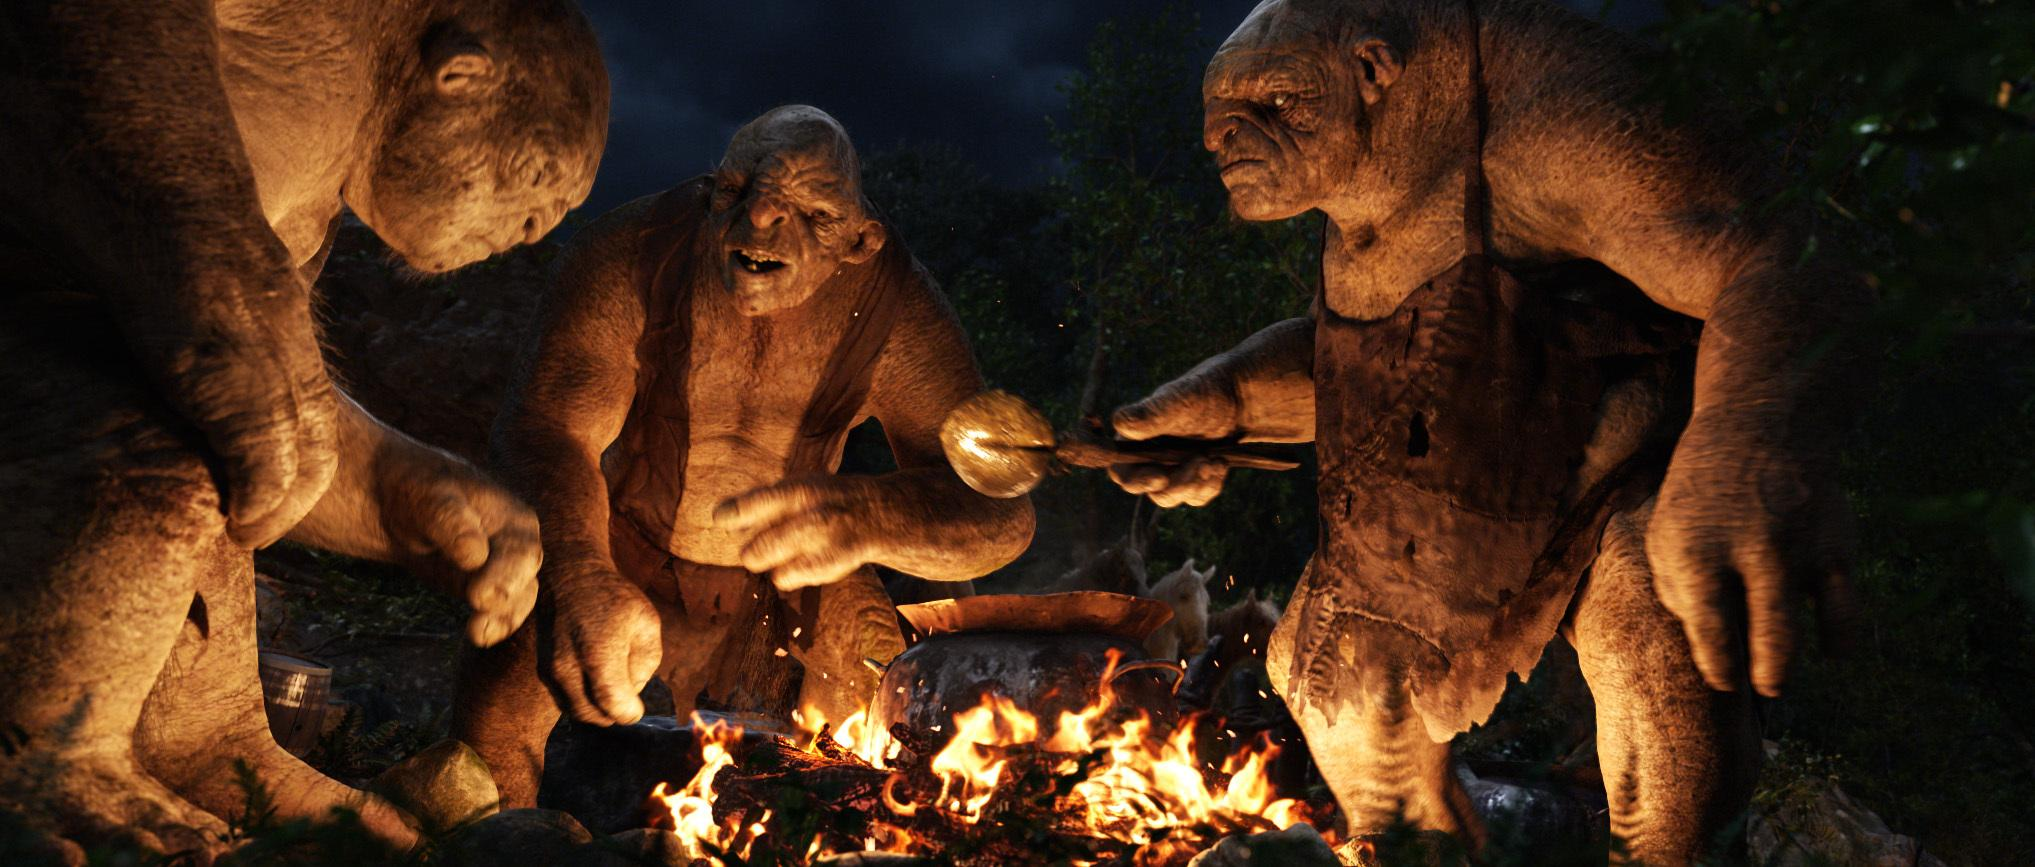
\includegraphics{hobbittrolls.jpg}}
%You've burnt the plot and added ingredients that the recipe didn't call
%for. This isn't Hobbit stew and you call yourself a chef.
%{[}/caption{]}

\captionsetup[figure]{labelformat=empty}
\begin{figure}[htbp]
\centering
\href{http://bakerjd99.wordpress.com/2012/12/16/king-hobbit-kong/hobbittrolls/}{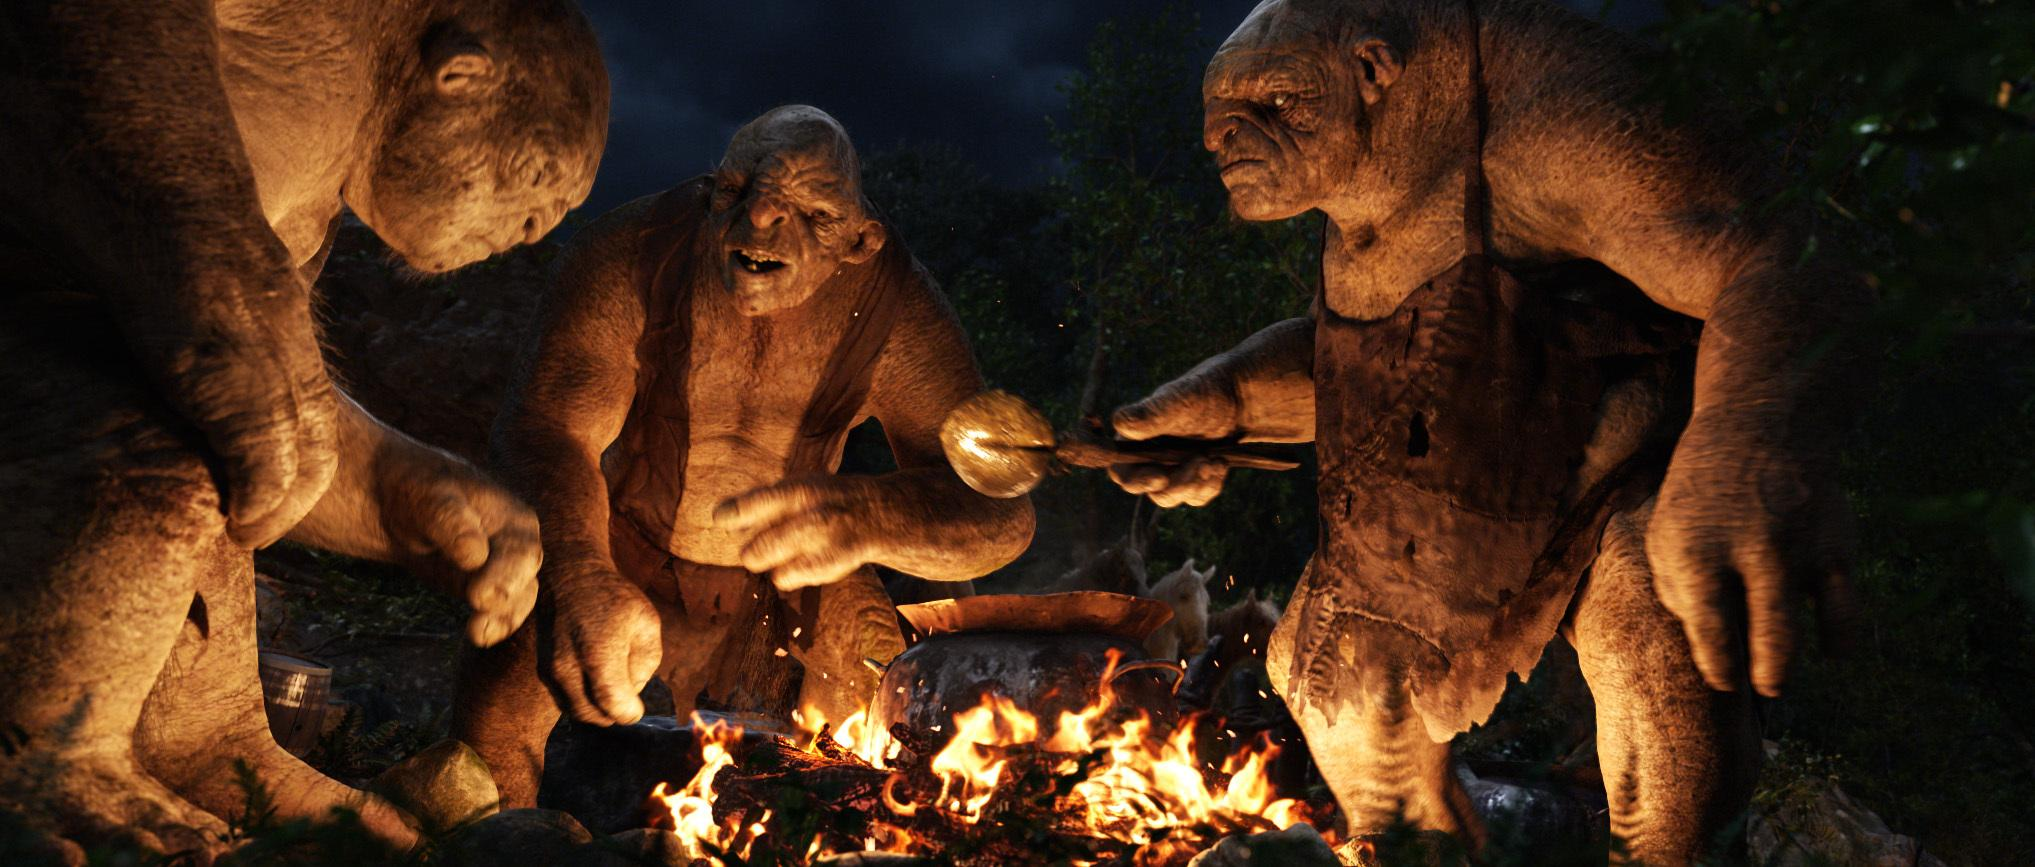
\includegraphics[width=0.70\textwidth]{hobbittrolls.jpg}}
\caption[This isn't Hobbit stew and you call yourself a chef]{You've burnt the plot and added ingredients that the recipe didn't call
for. This isn't Hobbit stew and you call yourself a chef.}
\label{fig:3538X0}
\end{figure}


%\captionsetup[floatingfigure]{labelformat=empty}
%\begin{figure}[htbp]
%\begin{floatingfigure}[l]{0.25\textwidth}
%\centering
%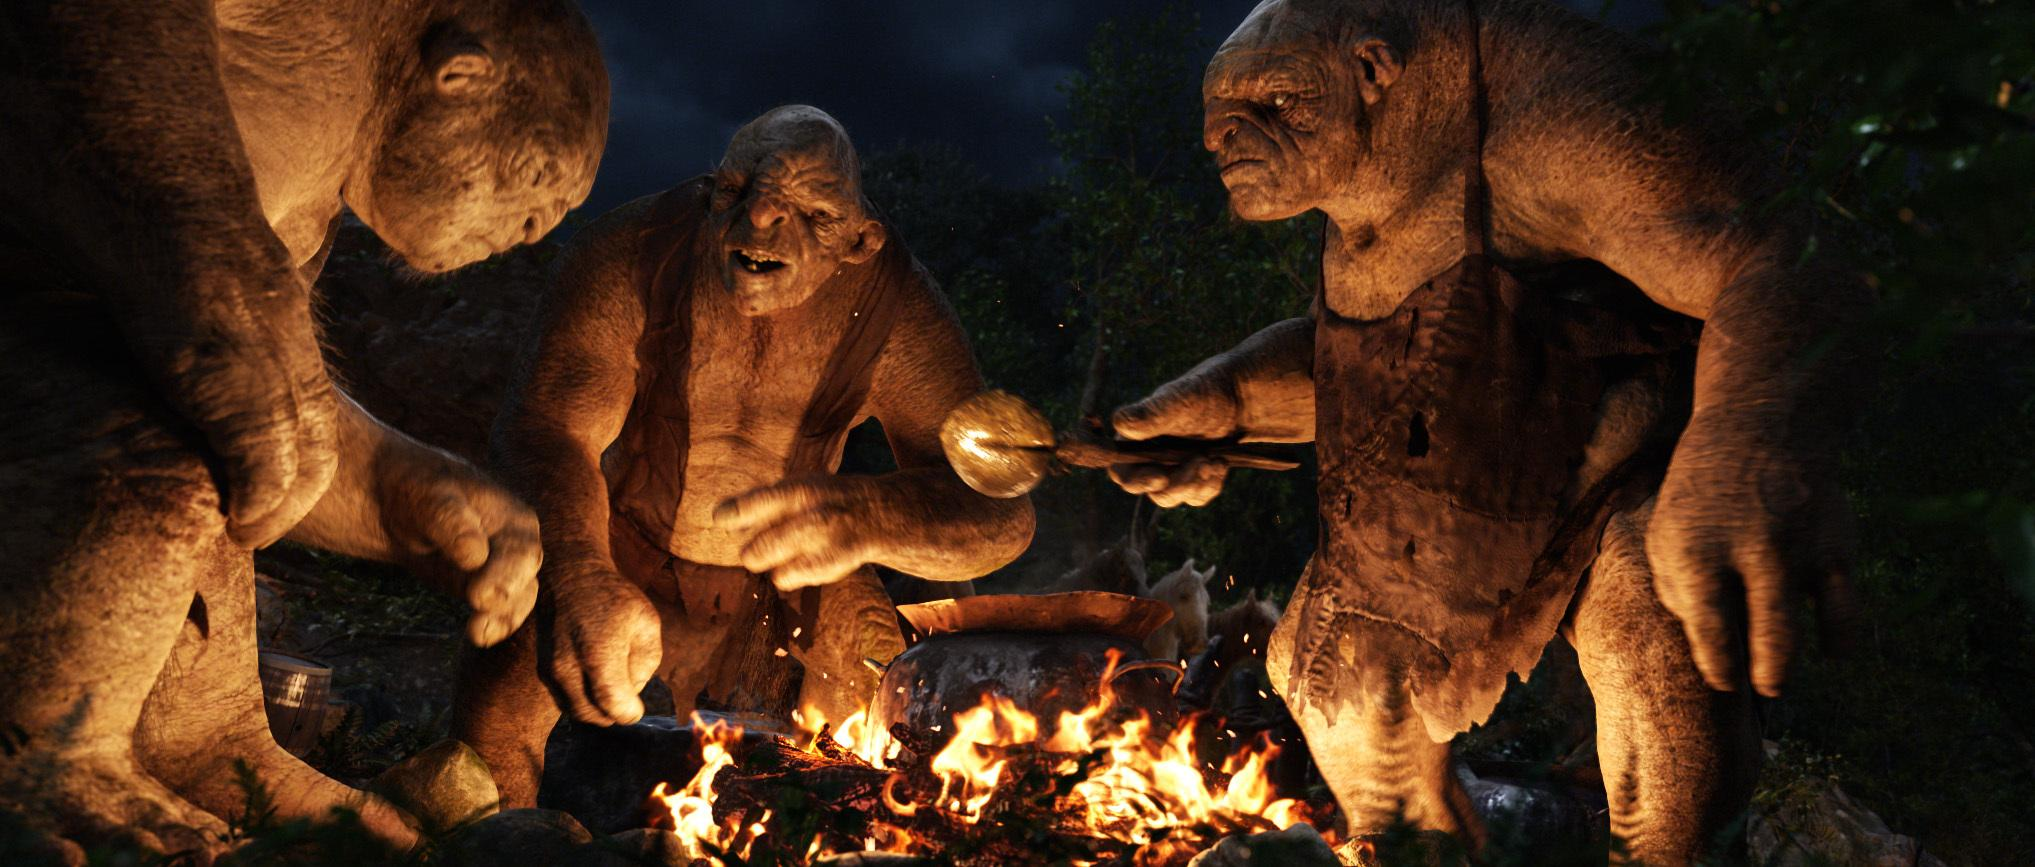
\includegraphics[width=0.23\textwidth]{hobbittrolls.jpg}
%\caption{~~~IMCAPTION~~~}
%\label{fig:3538X0}
%\end{floatingfigure}
%\end{figure}



%\end{document}